\documentclass[aspectratio=169, 14pt]{beamer}
\usepackage[utf8]{inputenc}
\usepackage{xeCJK}
\usepackage{graphicx}
\usepackage{transparent}
\usepackage[ruled, lined, linesnumbered, commentsnumbered]{algorithm2e}
\usepackage{pgfplots}
\usepackage{tikz}
\usetikzlibrary{matrix,backgrounds}
\usetikzlibrary{arrows}
\usetikzlibrary {arrows.meta}
\usetikzlibrary{calc,shadows.blur,fit,positioning}
\usepackage{minted}
\usepackage{fontawesome5}
\usepackage{booktabs}
\usepackage{caption}
\usepackage{hyperref}
\hypersetup{
    colorlinks=true,
    linkcolor=blue,
    filecolor=magenta,      
    urlcolor=cyan,
    }
\urlstyle{same}
\usetheme{metropolis}
\metroset{block=fill}
\usecolortheme{default}
\definecolor{darkmidnightblue}{rgb}{0.0, 0.2, 0.4}
\definecolor{LightGray}{gray}{0.9}


%------------------------------------------------------------
%This block of code defines the information to appear in the
%Title page
\title[Database Principles and Applications] %optional
{数据库原理与应用}

\subtitle{中级 SQL}

\author[CHEN Zhongpu] % (optional)
{CHEN Zhongpu}

\institute[] % (optional)
{
  School of Computing and Artificial Intelligence \\
  \href{mailto:zpchen@swufe.edu.cn}{zpchen@swufe.edu.cn}
}

\date[] % (optional)
{SWUFE, Fall 2022}

%End of title page configuration block
%------------------------------------------------------------


%------------------------------------------------------------
%The next block of commands puts the table of contents at the 
%beginning of each section and highlights the current section:

% \AtBeginSection[]
% {
%   \begin{frame}
%     \frametitle{Table of Contents}
%     \tableofcontents[currentsection]
%   \end{frame}
% }
%------------------------------------------------------------


\begin{document}

%The next statement creates the title page.
\frame{\titlepage}

%---------------------------------------------------------
%This block of code is for the table of contents after
%the title page
% \begin{frame}
% \frametitle{Table of Contents}
% \tableofcontents
% \end{frame}
%--------------------------------------------------------
\begin{frame}[fragile]
\frametitle{复习}
\begin{itemize}
    \item DDL (\texttt{create/drop/alter table})
    \item DML (\texttt{select, update, delete, insert})
\end{itemize}

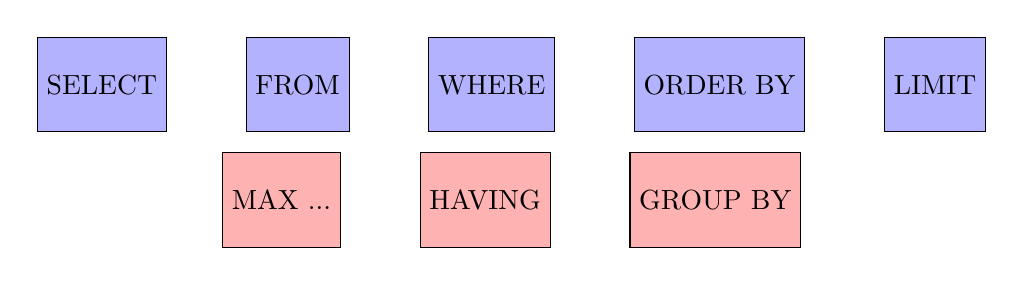
\begin{tikzpicture}[slot/.style={minimum size=1.2cm,rectangle, fill=blue!30},slot1/.style={minimum size=1.2cm,rectangle, fill=red!30},>=Stealth]
    \matrix [nodes=draw, row sep=0.2cm, column sep=1cm] (one) {
        \node[slot]{SELECT}; & \node[slot]{FROM}; & \node[slot]{WHERE}; & \node[slot]{ORDER BY}; & \node[slot]{LIMIT}; \\
    };
    \matrix [nodes=draw, row sep=0.2cm, column sep=1cm, below=of one, yshift=1cm] {
        \node[slot1]{MAX ...}; &
        \node[slot1]{HAVING};
        &\node[slot1]{GROUP BY};\\
    };

\end{tikzpicture}

\end{frame}

\begin{frame}[fragile]
    \frametitle{练习 (1)}
考虑大学数据库,找出 2017 年秋季 (Fall) 开设的每个课程段 (\texttt{section}) 的选课人数。(提示:仅考虑选课人数大于 0 的课程段,使用关系 \texttt{takes})

\pause
\begin{minted}[bgcolor=LightGray]{sql}
SELECT course_id, sec_id, count(id)
FROM takes
WHERE semester = 'Fall' AND year = 2017
GROUP BY course_id, sec_id;
\end{minted}

\end{frame}

\begin{frame}[fragile]
    \frametitle{练习 (2)}
考虑大学数据库,找出 2017 年秋季 (Fall) 开设的每个课程段 (\texttt{section}) 的选课人数。(提示:包括选课人数等于 0 的课程段,使用关系 \texttt{takes} 和 \texttt{section})

\pause
    
\begin{minted}[bgcolor=LightGray, baselinestretch=.9, fontsize=\small]{sql}
SELECT course_id, sec_id,
    (SELECT count(id)
        FROM takes
        WHERE takes.year = section.year
        AND takes.semester = section.semester
        AND takes.course_id = section.course_id
        AND takes.sec_id = section.sec_id)
FROM section
WHERE semester = 'Fall'
AND year = 2017;
\end{minted}

\end{frame}

{
    % \usebackgroundtemplate{\transparent{0.3}{\begin{picture}
    %     
\includegraphics[height=0.7\paperheight]{cover}
    % \end{picture}    
    % }}
\usebackgroundtemplate{
  \tikz[overlay,remember picture] 
  \node[opacity=0.3, at=(current page.south east),anchor=south east, yshift=2cm,xshift=4cm] {
    
\includegraphics[height=0.6\paperheight]{cover}};
}
    \begin{frame}
        \section{\textcolor{darkmidnightblue}{1. 连接 (Join)}}

        \begin{quote}
            A query that accesses multiple rows of the same or different tables at one time is called a \alert{join query}.            
        \end{quote}
    \end{frame}

}

\begin{frame}[fragile]
    \frametitle{1.1 自然连接 (natural join)}
找到学生名字及其所选课程 ID。   

\begin{itemize}
    \item \texttt{\textbf{takes}(ID, course\_id, sec\_id, semester, year, grade)}
    \item  \texttt{\textbf{student}(ID, name, dept\_name, tot\_cred)}
\end{itemize}
\[\Pi_{name, course\_id}(student \Join takes)\] 

\pause
\begin{minted}[bgcolor=LightGray, baselinestretch=1]{sql}
-- 相同名称属性的值相等
SELECT name, course_id
FROM student, takes
WHERE name.id = takes.id;
\end{minted}

\end{frame}

\begin{frame}[fragile]
通常我们考虑\textbf{所有相同名称属性上的相等}。SQL将其简化为「自然连接」(natural join):

    \begin{minted}[bgcolor=LightGray, baselinestretch=1]{sql}
SELECT name, course_id
FROM student, takes
WHERE student.id = takes.id;

-- 两种写法没有区别
SELECT name, course_id
FROM student NATURAL JOIN takes;
    \end{minted}

\pause
\textbf{思考}:没有选课的学生会出现在结果吗?(提示:\texttt{mydb} 中 Snow 没有选课)
\end{frame}

\begin{frame}[fragile]
    \frametitle{练习}

下面两条 SQL 语句的结果是否相同?
    
\begin{minted}[bgcolor=LightGray, baselinestretch=.9]{sql}
-- 笛卡尔积可以理解成 cross join
SELECT *
FROM student, takes
WHERE student.id = takes.id;

SELECT *
FROM student NATURAL JOIN takes;
\end{minted}

\pause
\begin{tikzpicture}
    \node[fill=yellow,blur shadow={shadow xshift=-0.5ex},
    text width=18em,anchor=south west,rounded corners]
    {自然连接只保留相同属性中的一个。};
\end{tikzpicture}  
\end{frame}

\begin{frame}[fragile]
    \frametitle{多个自然连接}
    \begin{minted}[bgcolor=LightGray, baselinestretch=1, fontsize=\small]{sql}
SELECT A1, A2, ..., An
FROM r1 NATURAL JOIN r2 NATURAL JOIN . . . NATURAL JOIN rm 
where P;
    \end{minted}
    
找到所有学生名字及其所选的课程名。

\begin{itemize}
    \item \texttt{\textbf{takes}(ID, course\_id, sec\_id, semester, year, grade)}
    \item \texttt{\textbf{student}(ID, name, dept\_name, tot\_cred)}
    \item \texttt{\textbf{course}(course\_id, title, dept\_name, credits)}
\end{itemize}

\end{frame}

\begin{frame}[fragile]

    \begin{minted}[bgcolor=LightGray, baselinestretch=1]{sql}
-- 正确
SELECT name, title
FROM student NATURAL JOIN takes, course
WHERE takes.course_id = course.course_id;

-- 错误
SELECT name, title
FROM student NATURAL JOIN takes NATURAL JOIN course;
    \end{minted} 

\pause
\begin{tikzpicture}
    \node[fill=yellow,blur shadow={shadow xshift=-0.5ex},
    text width=20em,anchor=south west,rounded corners]
    {要警惕自然连接中可能的不必要相等属性。};
\end{tikzpicture} 

\end{frame}

\begin{frame}[fragile]
    \frametitle{指定自然连接的属性}

\begin{tikzpicture}[framed, -stealth]
    \node (line) {\large{\textbf{自然连接}的条件是:\textcolor{red}{所有相同名称属性}上的相等。}};

    \node[below=of line] (using){\textcolor{red}{使用 \texttt{join $\dots$ using} 指定具体的属性}};

    \draw[ultra thick, draw=red] (line) -- (using);
\end{tikzpicture}

\begin{tikzpicture}
    \node[fill=yellow,blur shadow={shadow xshift=-0.5ex},
    text width=16em,anchor=south west,rounded corners]
    {\texttt{join $\dots$ using} 也会去除重复属性。};
\end{tikzpicture} 

\end{frame}

\begin{frame}[fragile]

    \begin{minted}[bgcolor=LightGray]{sql}
SELECT name, title
FROM student NATURAL JOIN takes, course
WHERE takes.course_id = course.course_id;

SELECT name, title
FROM (student NATURAL JOIN takes) 
    JOIN takes USING (course_id);
    \end{minted}
    
    \begin{tikzpicture}
        \node[fill=yellow,blur shadow={shadow xshift=-0.5ex},
        text width=20em,anchor=south west,rounded corners]
        {\texttt{using} 后面必须加括号,即使只有一个属性。};
    \end{tikzpicture} 

\end{frame}

\begin{frame}[fragile]
    \frametitle{1.2 join 的条件}

\begin{tikzpicture}[framed, -stealth]
    \node (line) {\large{\textbf{自然连接}的条件是:\underline{所有相同名称属性}上的\textcolor{blue}{相等}。}};

    \node[above=of line] (using){使用 \texttt{join $\dots$ using} 指定具体的属性};

    \draw[ultra thick] (line) -- (using);

    \node[below=of line, xshift=4cm] (on) {\textcolor{blue}{使用 \texttt{on} 指定任意条件}};

    \draw[ultra thick, draw=blue] (6, -0.3) -- (on);
\end{tikzpicture}

\textbf{思考}:使用 \texttt{on} 指定条件的连接是否会去除重复属性?

\end{frame}

\begin{frame}[fragile]
    \begin{minted}[bgcolor=LightGray, baselinestretch=1]{sql}
SELECT name, course_id
FROM student, takes
WHERE student.id = takes.id;

SELECT name, course_id
FROM student NATURAL JOIN takes;

SELECT name, course_id
FROM student JOIN takes USING (id);

SELECT name, course_id
FROM student JOIN takes
ON student.id = takes.id;
    \end{minted}

\end{frame}

\begin{frame}[fragile]
    \frametitle{练习}

将下面的查询使用 \texttt{join} 和 \texttt{on} 改写。

\begin{minted}[bgcolor=LightGray, baselinestretch=1]{sql}
SELECT DISTINCT T.name
FROM instructor AS T, instructor AS S
WHERE T.salary > S.salary
AND S.dept_name = 'History';    
\end{minted}

\pause

\begin{minted}[bgcolor=LightGray, baselinestretch=1]{sql}
SELECT DISTINCT T.name
FROM instructor AS T JOIN instructor AS S
ON T.salary > S.salary
WHERE S.dept_name = 'History';   
\end{minted}

\end{frame}

\begin{frame}[fragile]
    \frametitle{on vs. where}

    \begin{minted}[bgcolor=LightGray, baselinestretch=1]{sql}
SELECT DISTINCT T.name
FROM instructor AS T JOIN instructor AS S
ON T.salary > S.salary
WHERE S.dept_name = 'History';   
    \end{minted}

\textbf{思考}:\texttt{where} 的作用与 \texttt{on} 看起来差不多,为什么 SQL 会引入 \texttt{on} 子句?

\pause
\begin{tikzpicture}
    \node[fill=yellow,blur shadow={shadow xshift=-0.5ex},
    text width=26em,anchor=south west,rounded corners]
    {至少一个理由是:让 \texttt{on} 成为 \texttt{join} 独有的谓词(条件)表达式,使得代码可读性更好。};
\end{tikzpicture} 

\end{frame}

\begin{frame}[fragile]
    \frametitle{1.3 外连接 (outer join)}
    \begin{minted}[bgcolor=LightGray, baselinestretch=1]{sql}
-- 没有选课的学生不会出现在结果中
SELECT *
FROM student NATURAL JOIN takes;

-- 默认 join 就是 inner join
SELECT *
FROM student NATURAL INNER JOIN takes;
    \end{minted}

默认的连接是 \alert{inner} 的,而外连接 (\texttt{outer join}) 可以在结果中包括 \texttt{null},从而不丢失数据。

\end{frame}

\begin{frame}[fragile]
    \begin{tikzpicture}[thick]
    \node (inner){
        \begin{tikzpicture}[scale=0.6]
            \draw (0,0) circle (2cm);
            \draw (3,0) circle (2cm);
            \draw (0,0) node {A};
            \draw (3,0) node {B};
            \draw [clip](0,0) circle (2cm);
            \fill[yellow] (3,0) circle (2cm);
            \draw[black,thick] (0,0) circle(2cm);
            \draw[black,thick] (3,0) circle(2cm);
        \end{tikzpicture}
    };
    \node[above=of inner, align=left, yshift=-1cm]{\texttt{A INNER JOIN B}\\(相当于 \alert{A JOIN B})};

    \node[right=of inner, xshift=2cm] (left){
        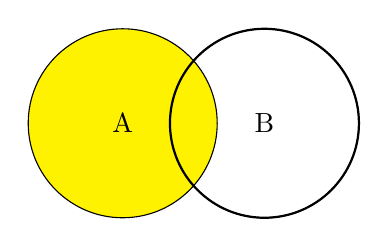
\begin{tikzpicture}[scale=0.6]
            \draw[fill=white] (3,0) circle (2cm);
            \draw[fill=yellow] (0,0) circle (2cm); 
            \draw[black,thick] (3,0) circle(2cm);
            \draw (0,0) node {A};
            \draw (3,0) node {B};
        \end{tikzpicture}
    }; 
    \node[above=of left, align=left, yshift=-1cm]{\texttt{A LEFT OUTER JOIN B}\\(相当于 \alert{A LEFT JOIN B})};

    \node[below=of inner, yshift=-1cm] (right){
        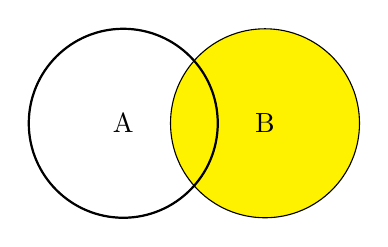
\begin{tikzpicture}[scale=0.6]
            \draw[fill=white] (0,0) circle (2cm);
            \draw[fill=yellow] (3,0) circle (2cm); 
            \draw[black,thick] (0,0) circle(2cm);
            \draw (0,0) node {A};
            \draw (3,0) node {B};
        \end{tikzpicture}
    }; 
    \node[above=of right, align=left, yshift=-1cm]{\texttt{A RIGHT OUTER JOIN B}\\(相当于 \alert{A RIGHT JOIN B})};

    \node[below=of left, yshift=-1cm] (full){
        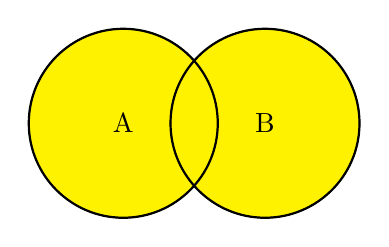
\begin{tikzpicture}[scale=0.6]
            \draw[fill=yellow] (0,0) circle (2cm);
            \draw[fill=yellow] (3,0) circle (2cm); 
            \draw[black,thick] (0,0) circle(2cm);
            \draw[black,thick] (3,0) circle(2cm);
            \draw (0,0) node {A};
            \draw (3,0) node {B};
        \end{tikzpicture}
    }; 
    \node[above=of full, align=left, yshift=-1cm]{\texttt{A FULL OUTER JOIN B}\\(相当于 \alert{A FULL JOIN B})};

    \end{tikzpicture}

\end{frame}

\begin{frame}[fragile]
    \frametitle{练习}
\begin{itemize}
    \item<1-> 如果要让尚未选课的学生出现在结果中,应该填入 \alert{left} 还是 \alert{right}?
    \begin{verbatim}
SELECT * 
FROM student () JOIN takes 
ON student.id = takes.id;
    \end{verbatim}
    \item<2-> 用自然连接 (\texttt{natural join}) 改写上面的查询。
\end{itemize}

\end{frame}

\begin{frame}[fragile]
    \frametitle{on vs. where (2)}
在外连接时,\texttt{on} 和 \texttt{where} 的作用不一样。

\begin{minted}[bgcolor=LightGray, baselinestretch=1]{sql}
SELECT *
FROM student LEFT JOIN takes
ON student.id = takes.id;

-- 未选课的学生不会出现
SELECT *
FROM student LEFT JOIN takes ON true
WHERE student.id = takes.id;
\end{minted}

\end{frame}

\begin{frame}
    \frametitle{小结}
    \begin{columns}
        \column{.4\textwidth}
        连接类型 (join types):
        \begin{itemize}
            \item \texttt{inner join}
            \item \texttt{left outer join}
            \item \texttt{right outer join}
            \item \texttt{full outer join}
        \end{itemize}
        \column{.6\textwidth}
        连接条件 (join conditions):
        \begin{itemize}
            \item \texttt{natural join}
            \item \texttt{on <predicate>}
            \item \texttt{using (A1, A2, ..., An)}
        \end{itemize}
    \end{columns}

\end{frame}
{\setbeamercolor{palette primary}{fg=black, bg=yellow}
\begin{frame}[standout]
    默认 \texttt{join} 是 \texttt{inner}

    有 \texttt{left/right/full},肯定是 \texttt{outer}

    \texttt{natural join} 是连接的条件,而不是类型

\end{frame}
}

\begin{frame}
    \frametitle{思考}

    部分数据库系统(如 MySQL)没有实现 \texttt{full outer join},只实现了 \texttt{left} 和 \texttt{right outer join}。那么如何在这样的数据库系统中写出 \texttt{full outer join}?

\end{frame}

\begin{frame}
    \frametitle{练习}
使用 \texttt{join} 找到所有老师的ID,以及他们所讲授课程段的总数,并且确保未上课的老师显示课程段总数显示为 0。(提示:使用关系 \texttt{instructor} 和 \texttt{teaches})

\begin{itemize}
    \item \texttt{\textbf{teaches}(ID, course\_id, sec\_id, semester, year)}
    \item \texttt{\textbf{instructor}(ID, name, dept\_name, salary)}
\end{itemize}
    
\end{frame}

\begin{frame}[fragile]

    \begin{minted}[bgcolor=LightGray, baselinestretch=1]{sql}
SELECT ID, count(sec_id)
FROM instructor NATURAL LEFT JOIN teaches
GROUP BY ID;

-- 使用标量子查询
SELECT ID,
       (SELECT count(*)
        FROM teaches T
        WHERE T.id = I.id)
FROM instructor I;
    \end{minted}
\end{frame}

\begin{frame}
    \section{\textcolor{darkmidnightblue}{2. 完整性约束 (续)}}
    包括:\texttt{primary key, foreign key, not null, unique, check}

\end{frame}

\begin{frame}[fragile]

    \begin{minted}[bgcolor=LightGray]{sql}
CREATE TABLE course
(   course_id    varchar(8), 
    title        varchar(50), 
    dept_name    varchar(20),
    credits      numeric(2,0) check (credits > 0),
    primary key (course_id),
    foreign key (dept_name) references department
);
    \end{minted}

\end{frame}

\begin{frame}[fragile]
    \frametitle{再谈外码}

考虑关系 \texttt{course}中的外码:

\begin{minted}[bgcolor=LightGray, baselinestretch=1]{sql}
foreign key (dept_name) references department 
\end{minted}

如果某学院(\texttt{department})被撤销,那么该学院开设的课程怎么办?
\pause
\begin{itemize}
    \item 默认是拒绝操作
    \item 对应课程都删掉(\alert{on delete cascade})
    \item 对应课程的学院名称设置为 \texttt{null}(\alert{on delete set null})
    \item 对应课程的学院名称设备为默认值 (\alert{on delete set default})    
\end{itemize}

\end{frame}

\begin{frame}[fragile]

    \begin{minted}[bgcolor=LightGray]{sql}
-- update 也有类似设置
CREATE TABLE course
(   course_id    varchar(8), 
    title        varchar(50), 
    dept_name    varchar(20),
    credits      numeric(2,0) check (credits > 0),
    primary key (course_id),
    foreign key (dept_name) references department
        on delete set null
);
    \end{minted}
\end{frame}

\begin{frame}
    \section{\textcolor{darkmidnightblue}{3. 视图 (view)}} 
    虚拟的表
\end{frame}

\begin{frame}[fragile]

    \begin{center}
        \begin{tikzpicture}[
            node distance=2cm,
            title/.style={font=\color{black!50}\ttfamily, fill=orange!30,},
            typetag/.style={rectangle, draw=black!50, font=\ttfamily, anchor=west}
          ]
            \node (decomp) [title] { \normalsize 视图层 (view level)};
          
            \node (di) [below=of decomp.west, typetag, yshift=0.5cm] { view 1 };
            \node (dr) [right=of di.west, typetag] { view 2 };
            \node (dots) [right=of dr.west] {...};
            \node (dnc) [right=of dots.west, typetag, xshift=-1cm] { view n };
          
            \node [draw=black!50,  fit={(decomp) (di) (dr) (dots) (dnc)}] (view){};
    
            \node[draw=black!50, below=of view, yshift=1cm,title](logical){逻辑层 (logical level)};
    
            \node[draw=black!50, below=of logical, yshift=1cm,title](physical){物理层 (physical level)}; 
    
            \draw[-, thick] (view) -- (logical);
            \draw[-, thick] (logical) -- (physical);
    
          \end{tikzpicture}
    \end{center}

\end{frame}

\begin{frame}[fragile]
    \frametitle{3.1 定义视图}
使用 \alert{create view} 命令:

\begin{verbatim}
CREATE VIEW v AS <query-expression>
\end{verbatim}
    
\begin{minted}[bgcolor=LightGray]{sql}
CREATE VIEW faculty AS
    SELECT ID, name, dept_name
    FROM instructor;
\end{minted}

\pause
\textbf{猜测}:删除视图定义的命令是什么?
\end{frame}

\begin{frame}
    \frametitle{3.2 使用视图}
\begin{itemize}
    \item<1-> 视图(view)并不预先计算并存储,而是在使用虚关系的时候才通过执行查询被重新计算处理。
    \item<1-> 从 SQL 查询语法上,「视图」和普通的「关系」没有区别。
    \item<2-> 部分数据库允许存储视图,并确保一旦关系发生改变,对应的视图也能更新。这样的视图叫物化视图 (materialized view)。
\end{itemize}

\pause
\textbf{练习}:利用 faculty 视图,查询 ID 为 10101 的教师信息。

\end{frame}

\end{document}